\documentclass[conference]{IEEEtran}

\usepackage{cite}
\usepackage[pdftex]{graphicx}
\graphicspath{{figures/}}
\usepackage[cmex10]{amsmath}
\usepackage{algorithmic}
\usepackage{array}
\usepackage{fixltx2e}
\usepackage{stfloats}
\usepackage{url}

\begin{document}

\title{Parallel Optimization for Stacked Autoencoders}

\author{\IEEEauthorblockN{Jason Liang}
\IEEEauthorblockA{jasonzliang@utexas.edu}
\and
\IEEEauthorblockN{Keith Kelly}
\IEEEauthorblockA{k3ithk@gmail.com}}

\maketitle

\begin{abstract}
The abstract goes here.
\end{abstract}

\section{Introduction}
introduction here

\begin{figure}[h]
\centering
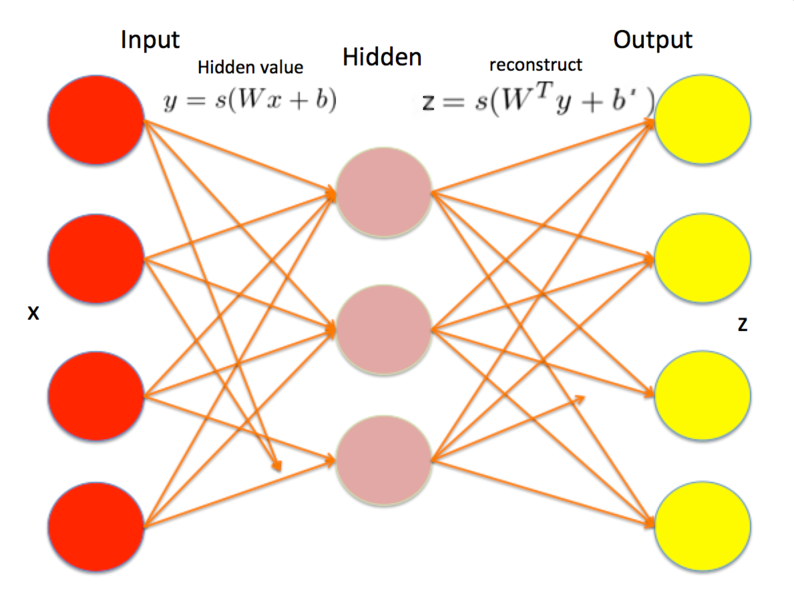
\includegraphics[width=0.9\linewidth]{autoencoder.png}
\caption{autoencoder}
\end{figure}

\section{Related Work}
related work here, cite like this \cite{vincent2010stacked}

\section{Algorithm Description}
describe SGD (backprop) for neural networks here

\section{Experimental Results}
experimental results here

\section{Future Work}
future work goes here

\section{Conclusion}
conclusion goes here

\bibliographystyle{unsrt}
\bibliography{autoencoder}

\end{document}


